\chapter{Final Project}

In this project we shall configure a network combining the different technologies that we have learned during this course. In particular, we shall extend the topology in the routing assignment with wireless connectivity (WLAN) and security (firewall) and traffic monitoring (Wireshark).

\section{Topology}

The topology that we will construct is presented in the figure \ref{fig:Final}. Similar to the routing assignments, each group will configure a part of the topology. In this assignment, each group will take care of a router, a firewall, a switch, an access point and the necessary computers. This topology interconnects secured networks (behind a firewall) with another network that offers access to the Internet. Each secured network needs at least one PC with an FTP server.

\begin{center}
\sffamily\small
\begin{tabular}{>{\columncolor{tablegray}}p{15cm}}
\multicolumn{1}{>{\columncolor{tablered}}l}{Important}\\
You should ask for the same firewall that you used during the firewall assignment.\\
\hline
Write down the UPF (or serial) number of your firewall and access point so you can identify them in the next session.\\
\hline
\end{tabular}
\end{center}

\begin{figure}
\centering
\ifpdf
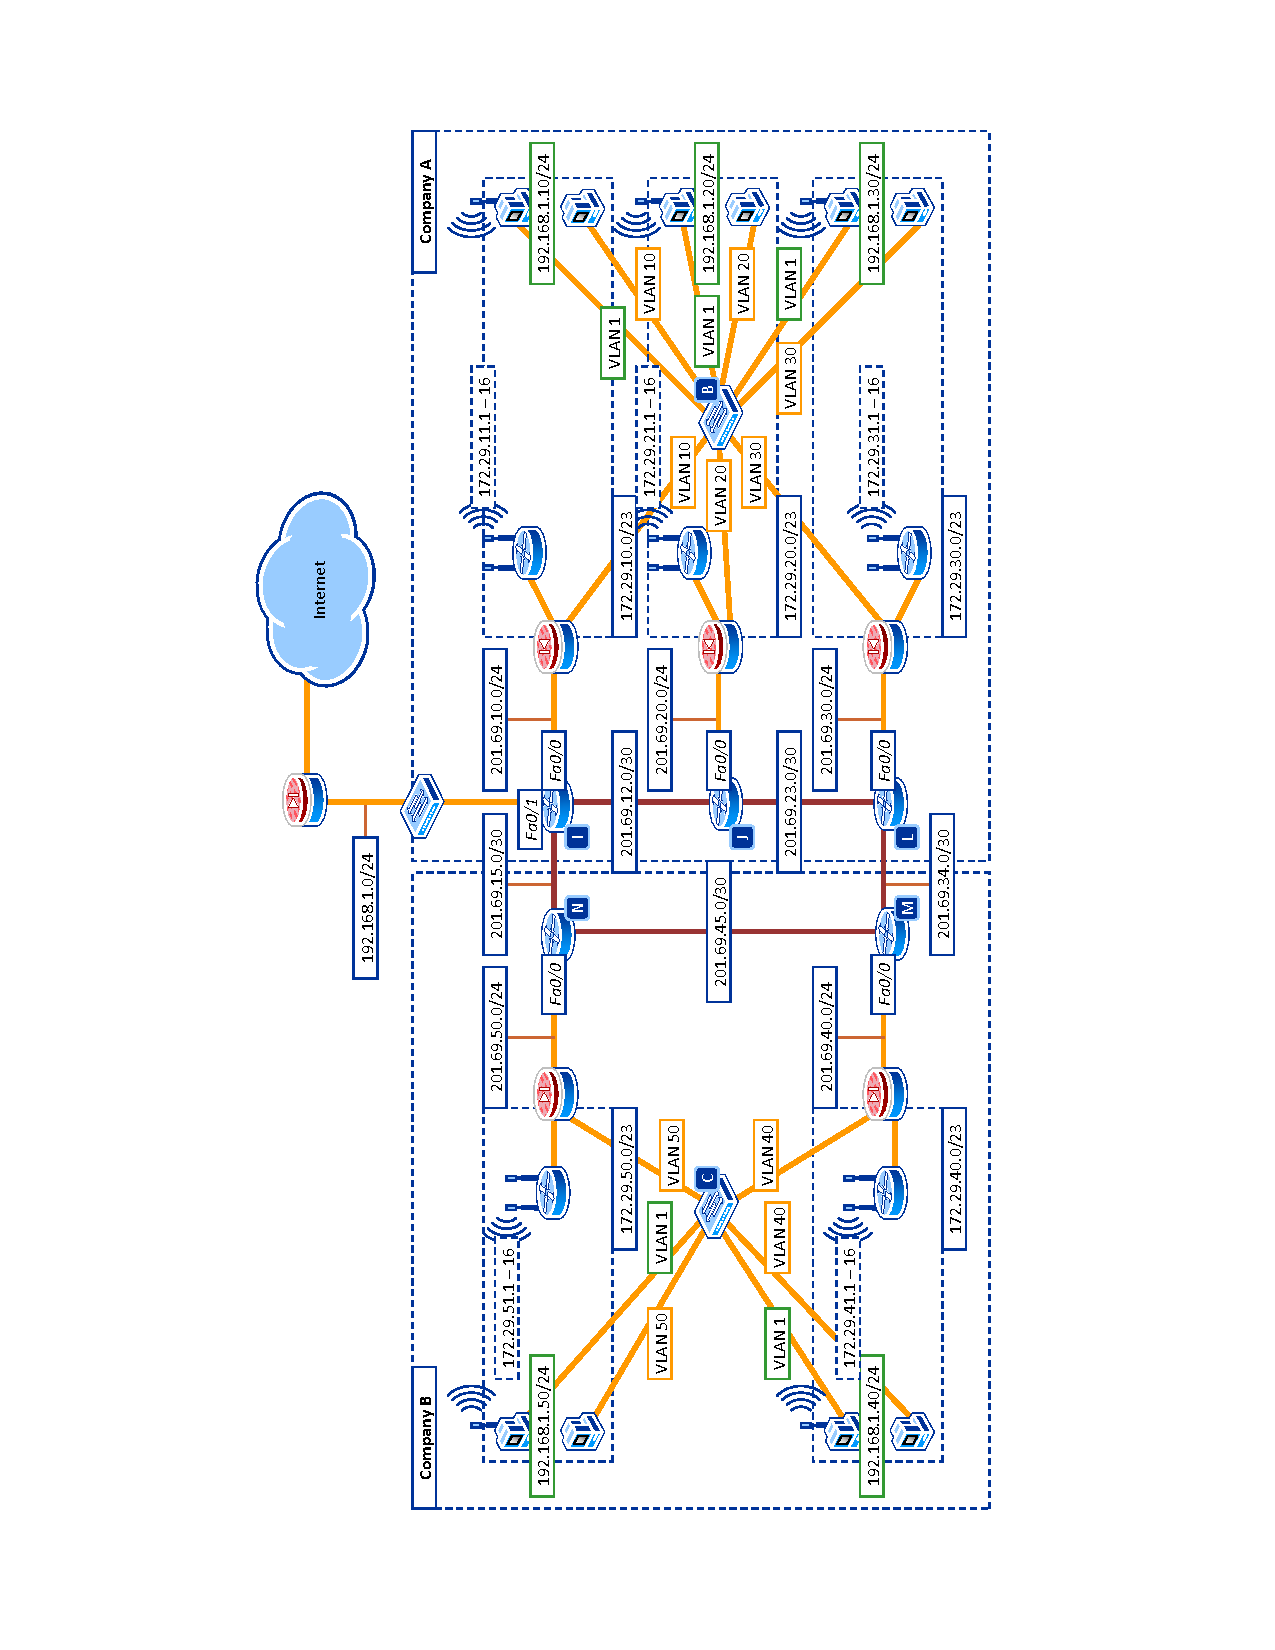
\includegraphics[width=0.9\linewidth]{Figures/Final.pdf}
\else
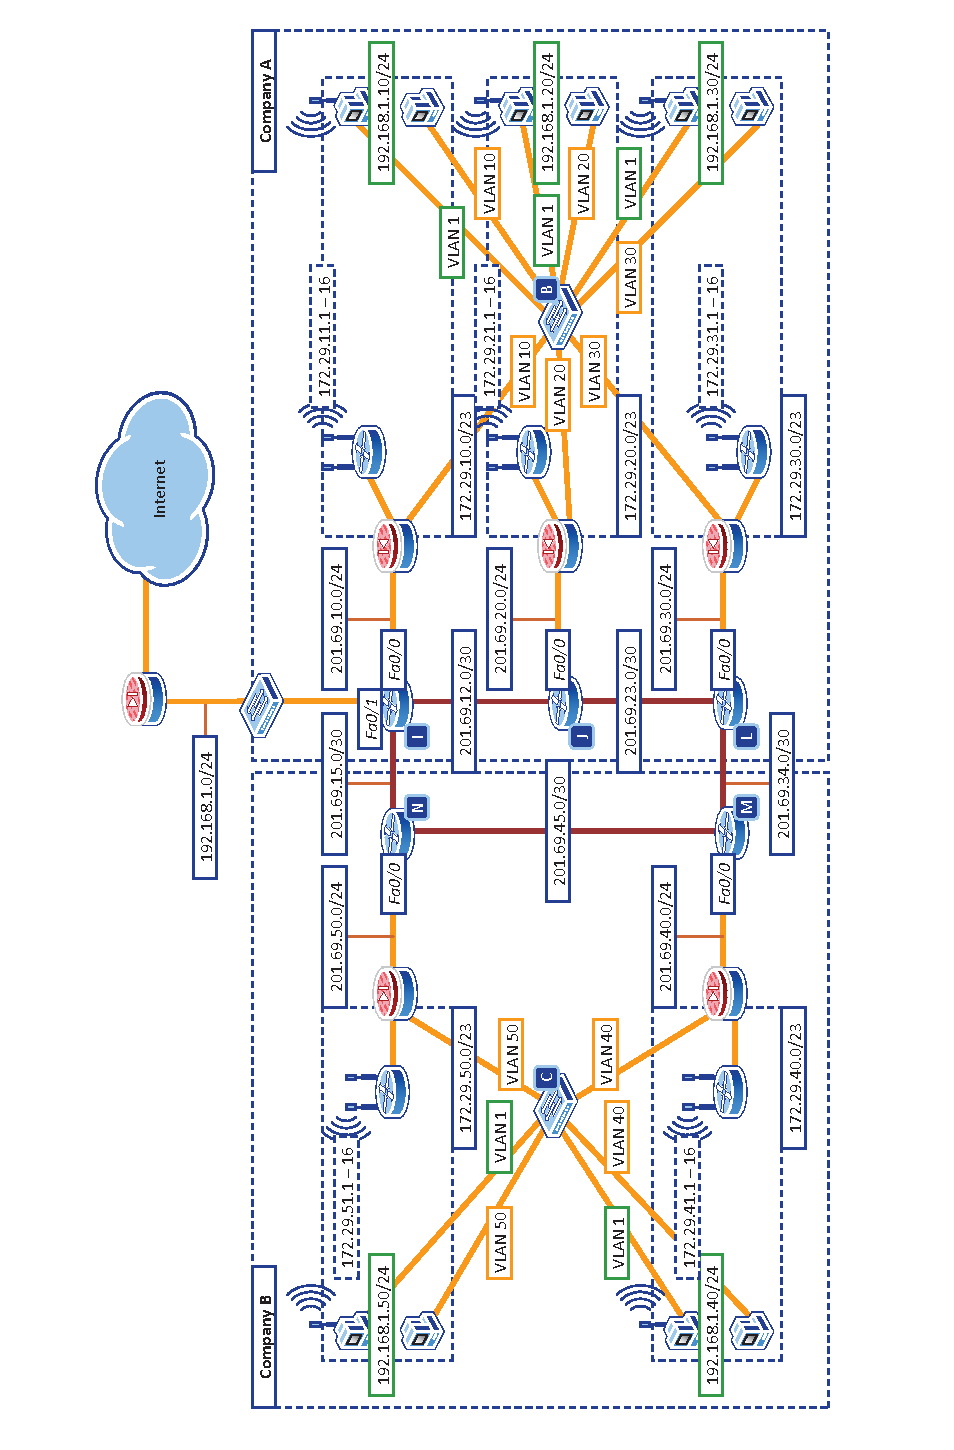
\includegraphics[width=0.9\linewidth]{Figures/Final.eps}
\fi
\caption{Topology of the final assignment}
\label{fig:Final}
\end{figure}

\section{Equipment and Addresses}

The assignment of equipment and addresses to the groups is detailed in the table \ref{tab:FinalEquipmentAndAddresses}. The switches are shared and the table specifies the ports for each group. The IP addresses for WLAN devices, Ethernet devices, the firewall interior interface and the public addresses are also included.

\begin{table}
\sffamily\small
\centering
\begin{tabular}{c>{\columncolor{tablegray}}c>{\columncolor{tablegray}}ccccccc}
\multicolumn{1}{>{\columncolor{tableheader}}c}{Group} & \multicolumn{1}{>{\columncolor{tableorange}}l}{Router} & \multicolumn{1}{>{\columncolor{tableorange}}l}{Switch} & \multicolumn{1}{>{\columncolor{tableheader}}c}{Ports} & \multicolumn{1}{>{\columncolor{tableheader}}c}{Public range} & \multicolumn{1}{>{\columncolor{tableheader}}c}{Private range} \\
1 & I & B & 1-8 & 201.69.10.0/24 & 172.29.10.0/23 \\
\hline
2 & J & B & 9-16 & 201.69.20.0/24 & 172.29.20.0/23 \\
\hline
3 & L & B & 17-24 & 201.69.30.0/24 & 172.29.30.0/23 \\
\hline
4 & M & C & 1-8 & 201.69.40.0/24 & 172.29.40.0/23 \\
\hline
5 & N & C & 9-16 & 201.69.50.0/24 & 172.29.50.0/23 \\
\hline
\end{tabular}
\caption{Equipment and addresses for the final assignment.}
\label{tab:FinalEquipmentAndAddresses}
\end{table}

Within each private subnetwork, we shall reserve the 172.29.X0.0/24 range for the Ethernet devices, and we shall use the 172.29.X1.0/24 range for the WLAN devices. We shall assign \emph{static} IP addresses to the computers using wired Ethernet connections, whereas the WLAN computers shall receive their IP address using \emph{DHCP}.

\section{Security Guidelines}

We shall imagine an enterprise scenario where we have to configure a network connecting two companies, A and B. Each team is configuring a company site, the number of sites being divided between the two companies.

The security guidelines are as follows:
\begin{itemize}
\item The internal computers should be able to connect to the internal FTP server.
\item The computers from other sites belonging to the \emph{same} company should be able to connect to the internal FTP server.
\item The computers from other sites belonging to the \emph{other} company should not be able to connect to the internal FTP server.
\item The computers should be able to ping external hosts.
\item It should not be possible for external hosts to ping internal computers.
\item All computers should have Internet connectivity.
\end{itemize}

\section{Device Configuration}

We have to configure the following devices at each site.

\begin{itemize}
\item \emph{Switch:} create the VLANs and assigning the corresponding ports.
\item \emph{Router:} configure the serial and Ethernet interfaces with the corresponding IP addresses, the routing protocol (RIPv1) and any needed static routes.
\item \emph{Access Point:} create a basic unsecured WLAN.
\item \emph{Firewall:} assign the IP addresses to the inside and outside interfaces, configure the DHCP server, security policy and NAT rules.
\end{itemize}

To configure the switch, you shall use an Ethernet port in VLAN\,1\footnote{Or alternatively, as your instructor may tell you.}.
To configure the router, you shall use the console connection.
To configure the firewall and the access point, you shall use the Ethernet ports.

\section{Home Preparation}

Find which ranges of IP are private addresses. Find information about Classless Inter-Domain Routing (CIDR) and what is the difference between /23 and /24 networks.

\begin{center}
\sffamily\small
\begin{tabular}{>{\columncolor{tablegray}}p{15cm}}
\multicolumn{1}{>{\columncolor{tableorange}}l}{Questions}\\
Do the addresses assigned to WLAN and ethernet devices belong to the same subnetwork? Why?\\
\hline
What is the explanation for the IP address for the internal interface of the firewall?\\
\hline
\end{tabular}
\end{center}

Fill in the figure \ref{fig:FinalAddresses} with your configuration information.

\begin{figure}
\centering
\ifpdf
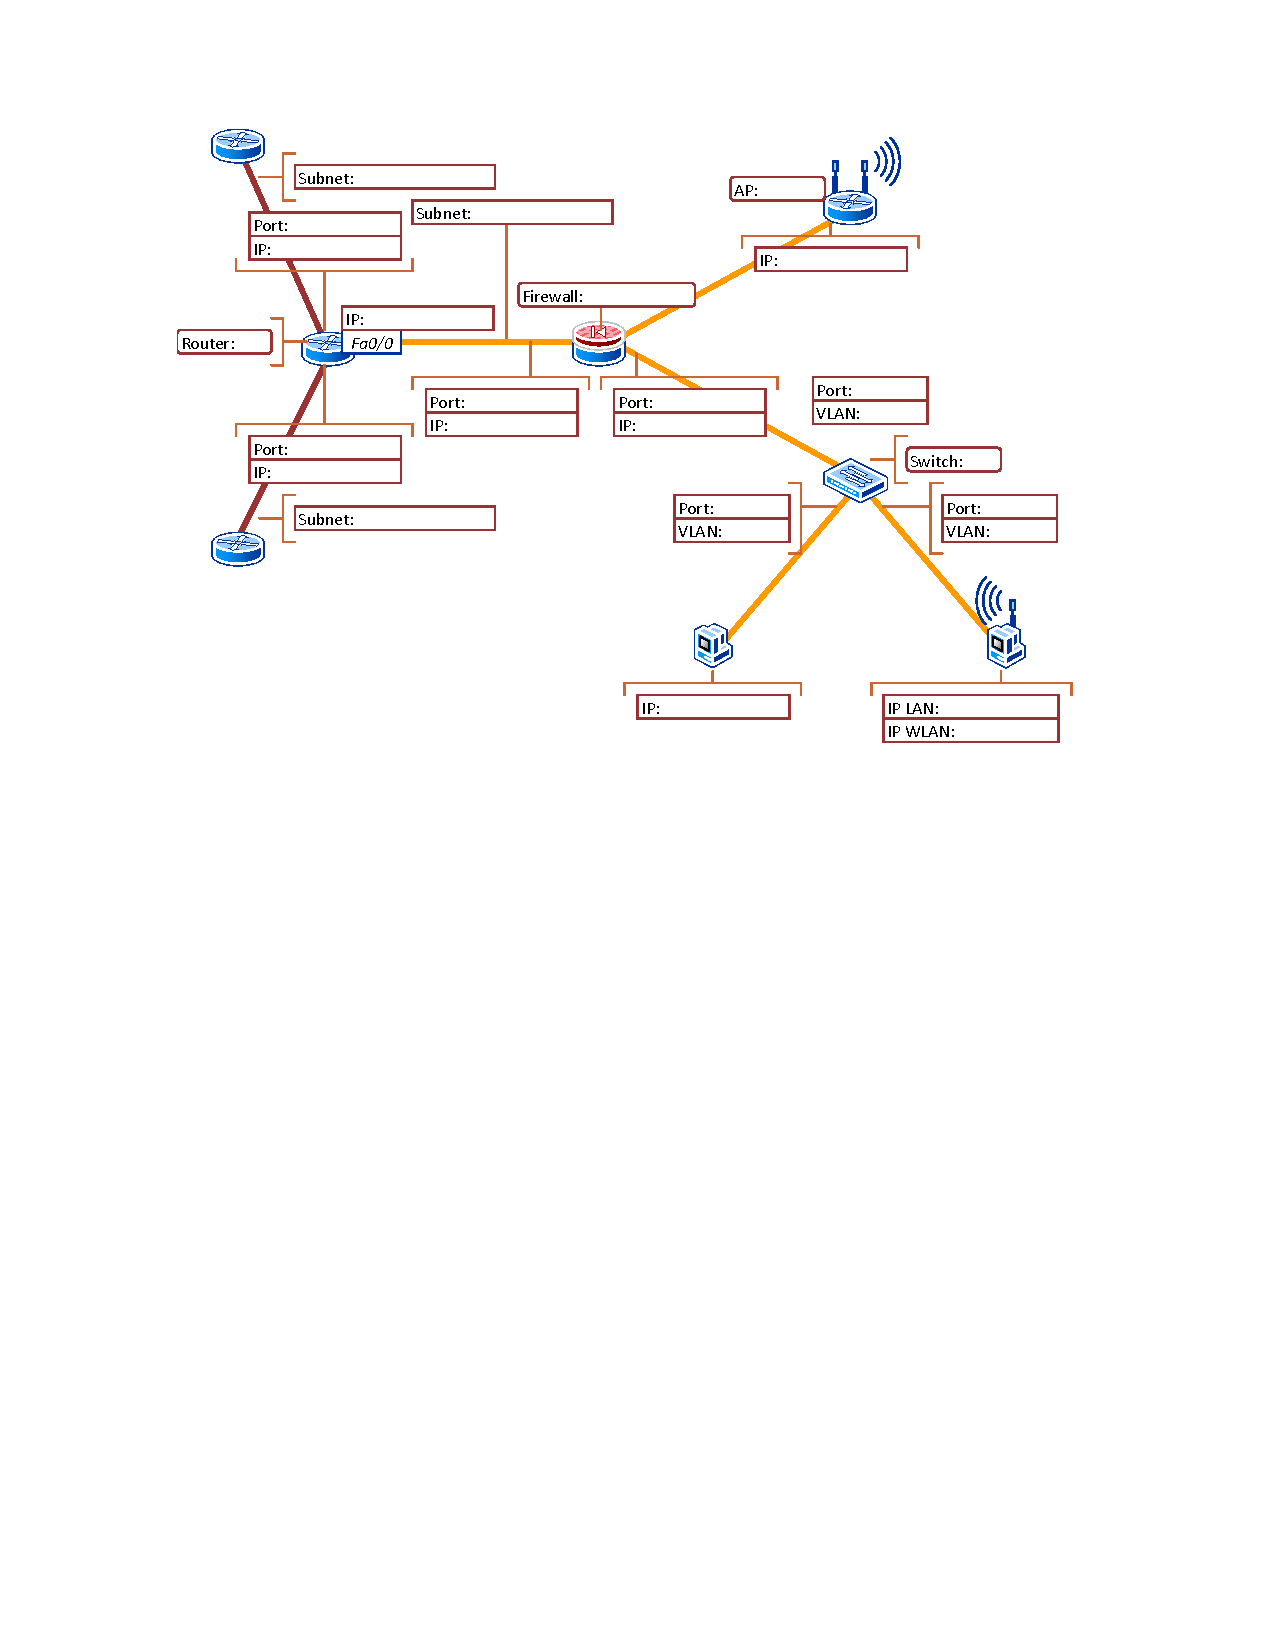
\includegraphics[width=0.9\linewidth]{Figures/FinalAddresses.pdf}
\else
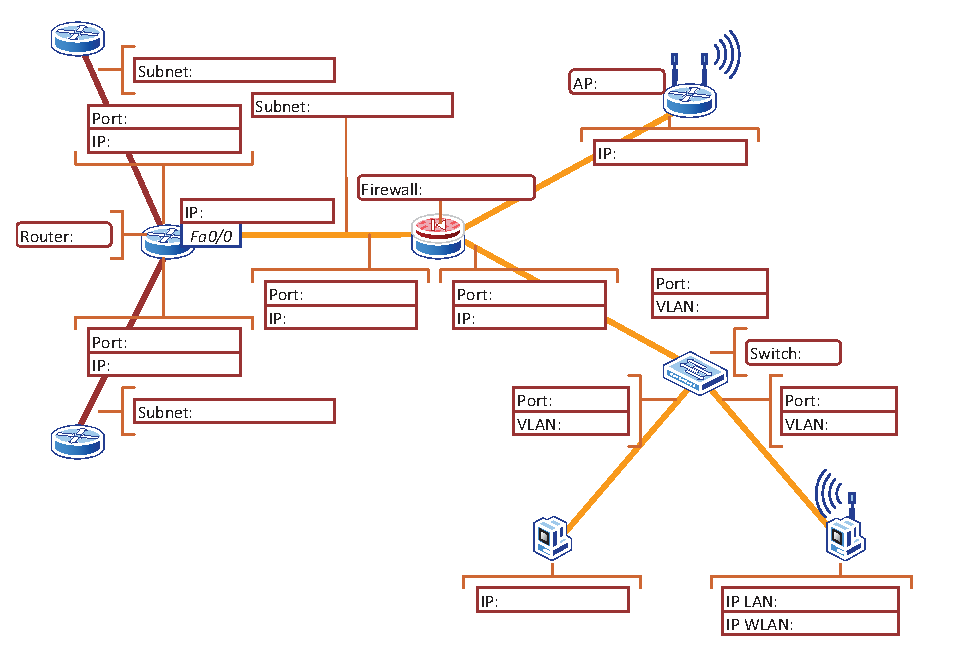
\includegraphics[width=0.9\linewidth]{Figures/FinalAddresses.eps}
\fi
\caption{Your configuration: equipments, ports and IP addresses.}
\label{fig:FinalAddresses}
\end{figure}

Fill in the figure \ref{fig:FinalFirewall} with your configuration information.

\begin{figure}
\centering
\ifpdf
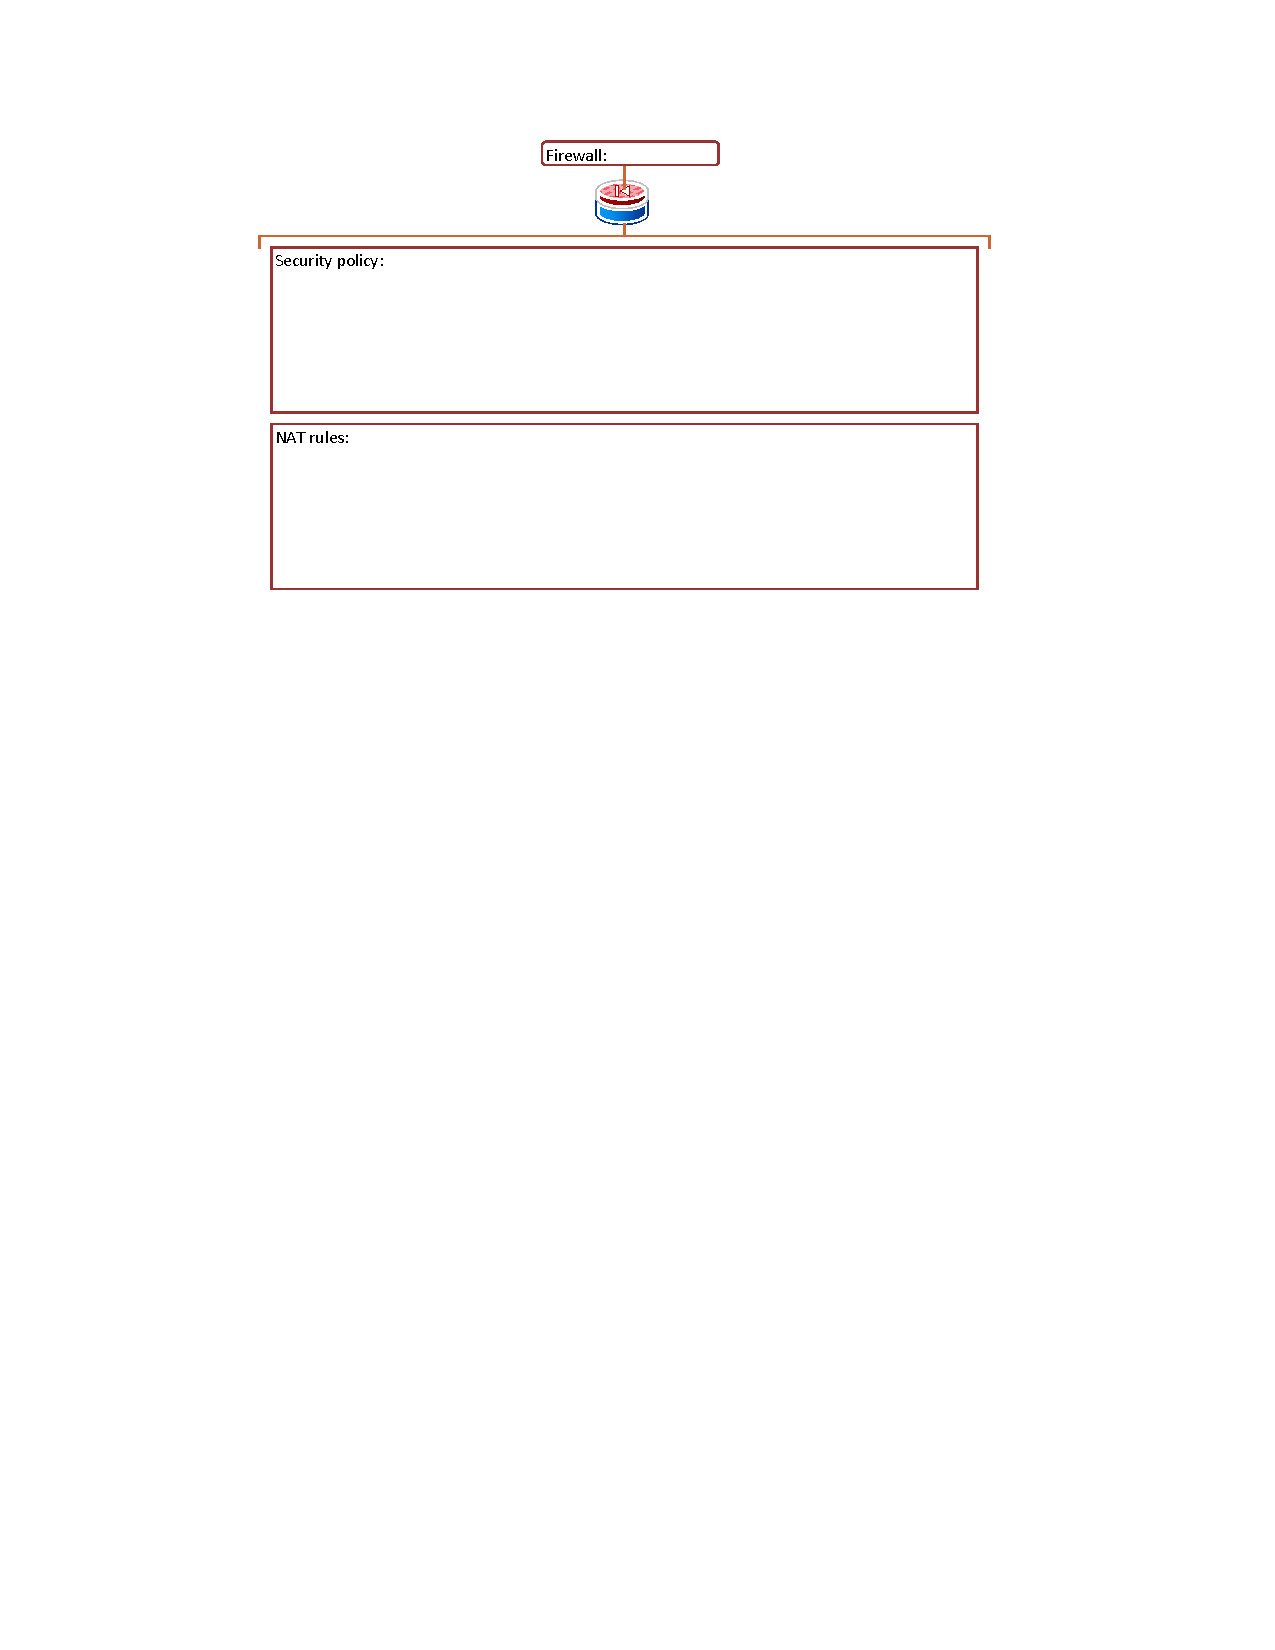
\includegraphics[width=0.9\linewidth]{Figures/FinalFirewall.pdf}
\else
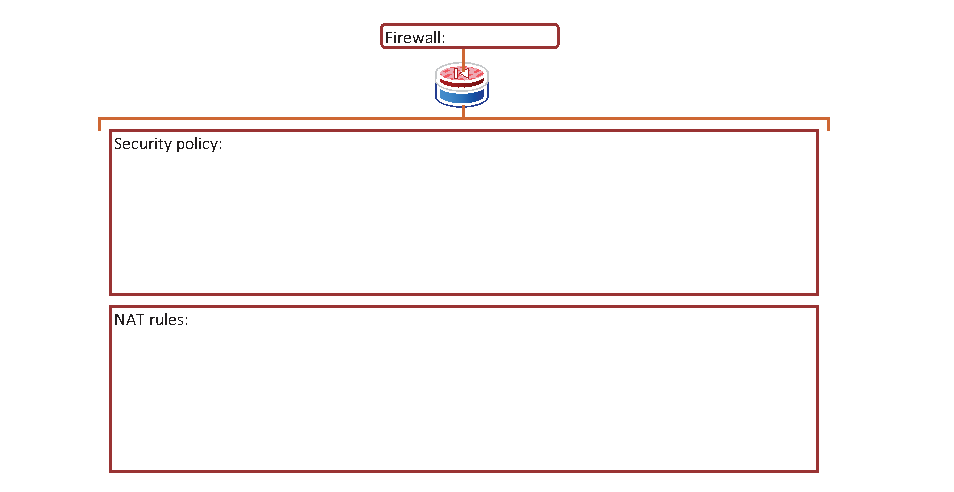
\includegraphics[width=0.9\linewidth]{Figures/FinalFirewall.eps}
\fi
\caption{Your firewall configuration: security policy and NAT rules.}
\label{fig:FinalFirewall}
\end{figure}


\section{Steps and Checkpoints for the Device Configuration}

\begin{enumerate}
\item \emph{Step:} Study the configuration.
\item \emph{Checkpoint:} Complete the configuration information in the figures above.
\item \emph{Step:} Configure the switches (VLANs and ports).
\item \emph{Checkpoint:} Check that the VLANs were created and the ports assigned.
\item \emph{Step:} Configure the internal wired computer and the firewall interfaces.
\item \emph{Checkpoint:} Ping the firewall from the internal computer.
\item \emph{Step:} Configure the router (interfaces and routing with RIP).
\item \emph{Checkpoint:} Ping from the router to the firewall, ping between routers, routing table, ping between firewalls.
\item \emph{Step:} Configure the firewall security policy and NAT rules.
\item \emph{Checkpoint:} Ping from the internal LAN computer to the routers. Can connect to the FTP servers from the other sites of the same company.
\item \emph{Step:} Configure the access point and firewall DHCP server.
\item \emph{Checkpoint:} Connect the internal wireless computer to the WLAN, and receive the IP configuration.
\end{enumerate}


\subsection{Switch Configuration}

The table \ref{tab:Final:Switch} contains the IP addresses for the switches.

\begin{table}
\sffamily\small
\centering
\begin{tabular}{>{\columncolor{tablegray}}ll}
\multicolumn{1}{>{\columncolor{tableorange}}c}{Switch} & \multicolumn{1}{>{\columncolor{tableheader}}c}{IP Address}\\
Switch B & 192.168.1.102 \\
\hline
Switch C & 192.168.1.103 \\
\hline
\end{tabular}
\caption{The IP addresses of the lab switches.}
\label{tab:Final:Switch}
\end{table}

\subsection{Computer Configuration}

The IP address of the DNS server is 193.145.56.11. On your wired computer in the 172.29.X0.0/23 subnetwork, install and configure an FTP server, with the username \texttt{groupX} and password blank, where $X$ is the number of your group.

\subsection{Firewall Configuration}

\begin{enumerate}
\item Connect the computer to the firewall on the \emph{inside} interface.
\item Enable HTTPS access to the network 172.29.X0.0, where $X$ is your group number.
\item Change the IP address of the \emph{inside} interface to 172.29.X0.1/23. After this change you shall lose connectivity to the firewall.
\item Change the IP address of the computer to 172.29.X0.2/23. The default gateway is the \emph{inside} interface of the firewall. Restart the ASDM.
\item Change the IP address of the \emph{outside} interface of the firewall to 201.69.X0.1/24.
\item Add a static default route at the outside interface of the firewall with your router interface as a gateway.
\end{enumerate}

\subsection{Router Configuration}

\begin{figure}
\centering
\ifpdf
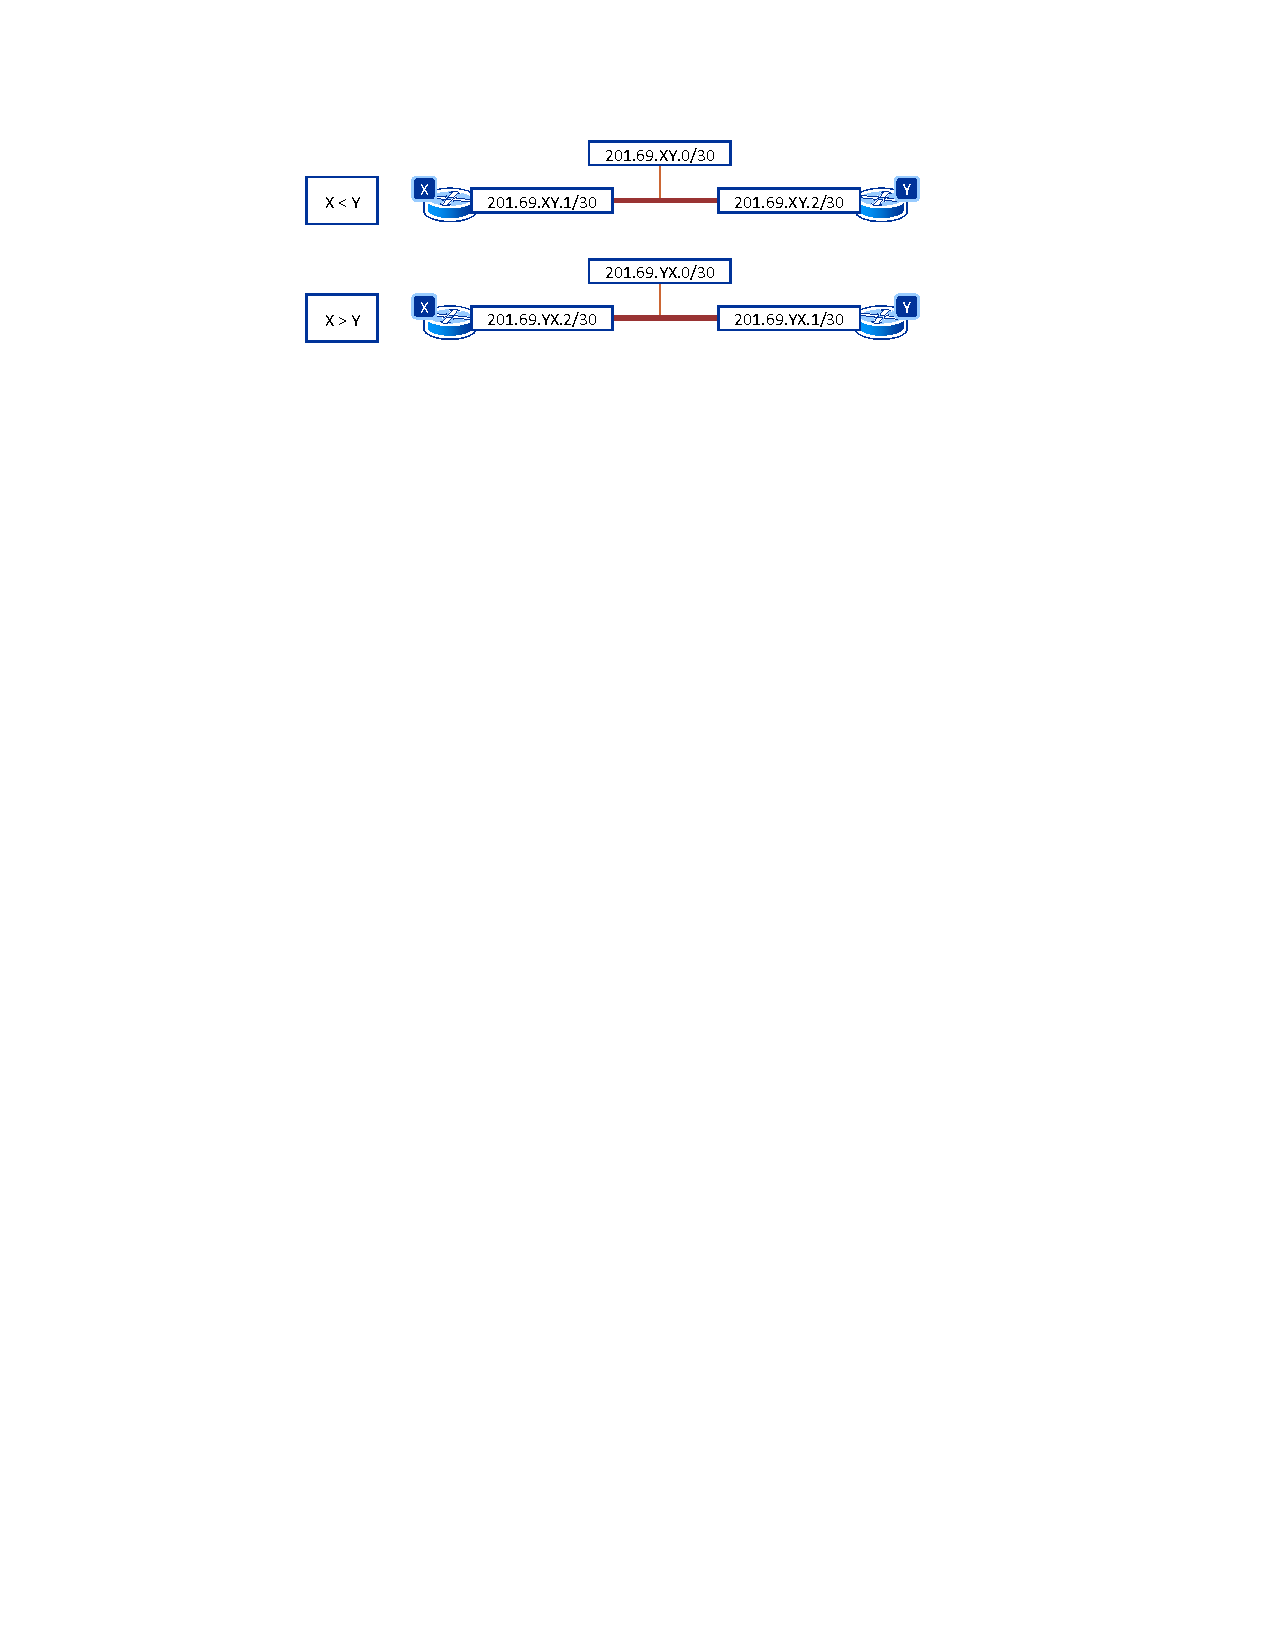
\includegraphics[width=0.9\linewidth]{Figures/FinalRoutersSerial.pdf}
\else
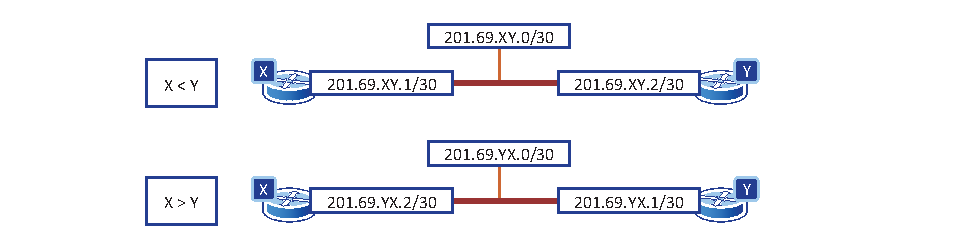
\includegraphics[width=0.9\linewidth]{Figures/FinalRoutersSerial.eps}
\fi
\caption{The IP addresses for the serial interfaces of two routers belonging to the groups $X$ and $Y$.}
\label{fig:FinalRoutersSerial}
\end{figure}

\begin{enumerate}
\item Configure the IP address of the Ethernet interface.
\item Configure the IP address of the serial interfaces. The IP addresses of a serial interfaces are assigned according to the figure \ref{fig:FinalRoutersSerial}. Do not forget to set the clock-rate to 128\,000 for all DCE interfaces.
\item Add RIP to the routing configuration. Add all networks. After convergence, check the routing table.
\item Configure the Internet access. Add an static route to the gateway of the lab, having the IP address 192.168.1.1
\end{enumerate}

\subsection{Access Point Configuration}

\begin{enumerate}
\item Change the IP of the access point and set the firewall as the default gateway.
\item Make sure that HTTP access is enabled.
\item Connect the access point to the firewall.
\item Use a computer with wired connection and the browser to connect to the access point. Configure the gateway. Configure the wireless network (enable the radio interface, SSID and security configuration).
\item Add a DHCP server to the firewall to provide an automatic configuration for the wireless computers. You can find the DHCP server configuration at \textsf{Configuration} \textgreater \textsf{Properties} \textgreater \textsf{DHCP Services} \textgreater \textsf{DHCP Server}. Configure the IP address range, the default gateway and the DNS.
\end{enumerate}

\subsection{Internet Gateway Configuration}

The IP address of the lab Internet gateway (firewall) is 192.168.1.1/24.

\section{Lab Report}

The lab report should include the devices configuration and the validation tests. As a minimum, it should contain the following.

\begin{enumerate}
\item The figures \ref{fig:FinalAddresses} and \ref{fig:FinalFirewall} completed with the required information. You may download the fillable forms for your lab reports at the following links:
\begin{itemize}
\item \url{http://alex.bikfalvi.com/teaching/upf/2013/networks_and_services/lab/final/FormAddresses.pdf}
\item \url{http://alex.bikfalvi.com/teaching/upf/2013/networks_and_services/lab/final/FormFirewall.pdf}
\end{itemize}

\item The configuration of the network equipments:
\begin{itemize}
\item The running configuration of your (i) \emph{router} and (ii) \emph{switch}.
\item A snapshot of the firewall (i) \emph{interfaces configuration}, (ii) \emph{security policy}, (iii) \emph{NAT rules} and (iv) \emph{DHCP configuration}.
\end{itemize}
\item Tables with results of the following validation tests (perform these tests \emph{after} all groups have finished their configuration):
\begin{itemize}
\item Ping between your wired and wireless computers.
\item Ping from your wired and wireless computers to all other routers.
\item Ping from your router to your wired and wireless computers.
\item Connect to your FTP server from the wireless computer.
\item Connect from the wired and/or wireless computer to the FTP server of another site from your company.
\item Connect from the wired and/or wireless computer to the FTP server of another site from the other company.
\item Connect to the Internet.
\end{itemize}
\end{enumerate}



\section{Optional Assignments}

Configure the firewall to prevent that wireless stations connect to the FTP server. Create a VPN between the sites of the same company.

